\section{Methodology}
\label{sec:method}

This section first describes our experimental design and setup. Then we briefly present the datasets, the data deletion strategies, and our evaluation metrics. 

\begin{figure*}[t!]
  \centering
  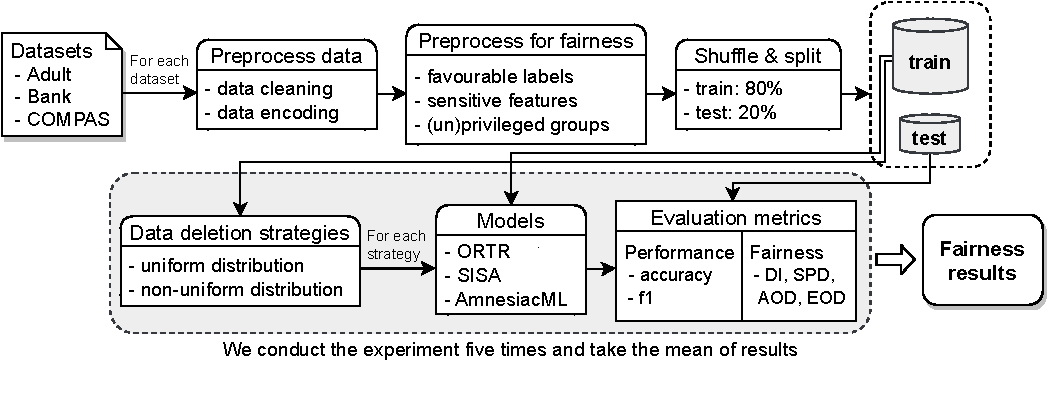
\includegraphics[scale=0.8]{assets/flowchart_ver9.pdf}
  \caption{Experimentation to evaluate the performance and fairness of machine unlearning methods under different scenarios. 
  }.
  \label{fig:design}
\end{figure*}

\subsection{Experiment Design}
\label{sec:design}

Our empirical study starts by first collecting the benchmark fairness datasets. For each dataset, we preprocess and split it into training and testing datasets. The training dataset is then employed to train machine unlearning models. We use six evaluation metrics to measure the performance and fairness of these models. Figure~\ref{fig:design} briefly presents an overview framework of our experimental design. 

To identify the fairness datasets, we first refer to the work on fairness testing for machine learning models that employed six datasets, such as German Credit, Adult, Bank, US Executions, Fraud Detection, and Raw Car Rentals~\cite{aggarwal2019black}. Among these datasets, only German Credit, Adult, and Bank are available. We also collect the Heart Disease dataset~\cite{heart}, referring to the presence of heart disease in patients, and the COMPAS dataset~\cite{compas}, aiming to predict the probability of criminals reoffending. In total, we acquire five datasets, i.e., German Credit, Adult, Bank, Heart Disease, and COMPAS, across various domains. As machine unlearning methods are efficient and effective on large datasets~\cite{sisa, amnesiac}, we remove datasets that have fewer than 1,000 instances including German Credit and Heart Disease. Hence, there are three datasets, i.e., Adult, Bank, and COMPAS, that are employed to evaluate the impacts of machine unlearning methods in our experiments. 

We apply the same data preprocessing approach for all three datasets. Specifically, we employ the AI Fairness 360 toolkit~\cite{aif360}, which is an open-source library for fairness metrics, to clean up invalid or missing values, transform categorical values into a one-hot encoding, and convert non-numerical binary values to a binary label (e.g., \textit{male}: 1, \textit{female}: 0). We further preprocess the datasets to employ them for fairness evaluation. Specifically, we specify favourable labels or the predicted outcome of our model. We also identify sensitive features (or protected classes) for the privileged and unprivileged groups.
For example, in the Adult dataset, the prediction label is a favourable label, indicating whether a person has a high annual salary. We define \textit{sex} as a sensitive feature. We assume that a \textit{male} often has a higher annual salary than a \textit{female}; hence, the \textit{male} should be put in the privileged group while the \textit{female} should be in the unprivileged group regarding the sensitive feature \textit{sex}. 
For each dataset, we shuffle and split it into the training dataset (80\%) and the testing dataset (20\%). We then feed the training dataset into our models. 

To conduct our experiments, we employ a multilayer perceptron (MLP), a simple feedforward network~\cite{ramchoun2016multilayer}. The MLP model includes an input layer, a hidden layer, and an output layer. We train the MLP model by optimizing a cross-entropy loss function~\cite{martinez2018taming}. Two machine unlearning methods, such as SISA and AmnesiacML, are built based on the MLP model. A na\"ive approach of using original training and retraining (denoted as \textbf{ORTR}) is also built based on the MLP model as the baseline. We consider two experimental scenarios. 

\begin{itemize} [leftmargin=*]
    \item \textbf{Scenario 1:}
    Before any ``\textit{right to be forgotten}'' (RTBF) requests, what are the impacts of machine unlearning methods on fairness? In this setting, the training dataset is put into three different models, such as ORTR, SISA, and AmnesiacML (see Figure~\ref{fig:design}), to train these models. We then employ the testing dataset to evaluate the performance and fairness of these trained models. 
    \item \textbf{Scenario 2:} When the RTBF requests arrive, what are the impacts of machine unlearning methods on fairness? In this setting, we employ data deletion strategies (see Figure~\ref{fig:design}) to remove instances from the training dataset. For each data deletion strategy, we compare the performance and fairness of ORTR with two machine unlearning methods, such as SISA and AmnesiacML. 
\end{itemize}





For each dataset, we apply 5-fold cross-validation and take the mean of the results. We have conducted our experiments using an Nvidia T4 GPU and an Intel Xeon Silver 4114 CPU with 16 GB RAM and 12 GB RAM, respectively. The OS is Debian 10.10 LTS 64 bit. The machine learning framework is PyTorch v.1.12 with CUDA 11.3, and the Python language version is 3.7. 


\subsection{Datasets}
\label{sec:data}



We conduct our experiments by employing three widely-used fairness datasets to evaluate the impacts of machine unlearning methods on fairness. These datasets are briefly described as follows. 

\begin{itemize} [leftmargin=*]
    \item \textbf{Adult}~\cite{adult}. This dataset is extracted from the 1994 Census Bureau database\footnote{https://www.census.gov/programs-surveys/ahs/data/1994.html}. Its task is to predict whether a person can earn over \$50,000 USD per year. The dataset includes 48,842 instances and 14 features. The sensitive features for this dataset are \textit{sex} and \textit{race}. 
    \item \textbf{Bank}~\cite{bank}. The dataset is collected from marketing campaigns of a Portuguese banking institution. Its task is to predict whether a client will subscribe to a bank term deposit. The dataset contains 45,211 instances and 17 features. We use \textit{age} as the sensitive feature for this dataset.
    \item \textbf{COMPAS}~\cite{compas}. The dataset contains recidivism records, which are used to build a prediction system to forecast the possibility of a criminal defendant reoffending. The dataset has 7,215 instances and seven features. The sensitive features are defined as \textit{sex} and \textit{race}.
\end{itemize}

All the sensitive features are selected by following the previous work~\cite{biswas2020machine, chakraborty2020fairway, zhang2021ignorance}.



 

\subsection{Data Deletion Strategies}
\label{sec:data_deletion}

To send the ``\textit{right to be forgotten}'' (RTBF) requests, we adopt two data deletion strategies. Each strategy has various settings presented as follows.


\noindent {\textbf{Uniform distribution.}} For this strategy, we assume that the deleted data has a uniform distribution, i.e., each instance has an equal probability of being removed from the training dataset. To select a range of proportions of the total amount of deleted data, we leverage the work of Bertram et al~\cite{rtbf5years}. Specifically, we randomly remove 1\%, 5\%, 10\%, and 20\% of the training data. 

\noindent {\textbf{Non-uniform distribution.}} For this strategy, we assume that the deleted data has a non-uniform distribution, i.e., each instance has a different probability of being removed from the training dataset. Some people have a higher probability of sending RTBF requests compared to other people. For example, people who are from wealthy families or have a high educational background prefer to keep their sensitive information private for security and privacy purposes~\cite{upton2001strategic, eurobarometer}. 
As these personal details are unavailable in our datasets, to better understand the fairness implications under different cases when the deleted data is a non-uniform distribution, we first assume that the people who request the RTBF are predominantly from privileged groups, and we assume another scenario that people exercising the RTBF are predominantly from unprivileged groups.




\subsection{Evaluation Metrics}
\label{sec:metrics}

We consider two types of evaluation metrics in our experiments, which are performance and fairness. 

\noindent \textbf{Performance measure.} Before evaluating the fairness of models, we calculate their performance in terms of accuracy and F1 score. 

\begin{itemize} [leftmargin=*]
    \item \textit{Accuracy:} The ratio of true predictions among the total number of predictions~\cite{gunawardana2009survey}.
    \item \textit{F1 score:} The harmonic mean between precision and recall~\cite{dalianis2018evaluation}.
\end{itemize}

\noindent \textbf{Fairness measure.} To measure the fairness of models, we adopt the four fairness metrics, i.e., disparate impact (DI), statistical parity difference, average odds difference, and equal opportunity difference, briefly mentioned in Section~\ref{sec:ai_metrics}. For simplicity in presenting and observing, we convert all the fairness metric values into their absolute values. As disparate impact (DI) value differs from other fairness metrics, we use $|$1 - DI$|$ to evaluate the fairness of our models. In this case, all four fairness metrics achieve the greatest fairness when their values equal 0.  


